\documentclass[a4paper, czech]{article}

\usepackage[czech]{babel}
\usepackage{indentfirst}
\usepackage{graphicx}
\usepackage{float}
\usepackage[margin=1.5cm]{geometry}
\usepackage{booktabs}
\usepackage{amsmath}
\usepackage[table]{xcolor}
\usepackage{multirow}
\usepackage{tabularray}
\usepackage{bold-extra}
\usepackage{gensymb}

\begin{document}
\begin{table}[H]
    \centering
    \begin{tblr}{
        cell{1}{1} = {c = 2, r = 4}{c}, % Logo
        cell{1}{4} = {c = 3}{c}, % Předmět
        cell{2}{4} = {c = 3}{c}, % Jméno
        cell{3}{4} = {}{c}, % Ročník
        cell{3}{6} = {}{c}, % Studijní skupina
        cell{4}{4} = {}{c}, % Spolupracoval
        cell{4}{6} = {}{c}, % Mereno dne
        cell{5}{1} = {c = 2}{55mm}, % Kontroloval
        cell{5}{3} = {c = 2}{55mm}, % Hodnoceni
        cell{5}{5} = {c = 2}{55mm}, % Dne
        cell{6}{2} = {c = 5}{}, % Nazev ulohy
        cell{7}{1} = {}{c}, % Číslo úlohy
        cell{7}{2} = {c = 5}{c}, % Název úlohy
        vline{1,2,7} = {1.2pt},
        vline{3,5},
        hline{1,5,6,8} = {1.2pt},
        hline{2,3,4}
        }
        
\includegraphics{logo_fekt.png} & & \textsuperscript{Předmět} & \large \textbf{Měření v audiotechnice} \\
             & & \textsuperscript{Jméno} & \large \textbf{Karolína Šebestová} \\
             & & \textsuperscript{Ročník} & \large \textbf{3.} & \textsuperscript{Studijní skupina} & \large \textbf{St 14:00} \\
             & & \textsuperscript{Spolupracoval} & \large \textbf{Filip Kokavec} & \textsuperscript{Měřeno dne} & \large \textbf{16.10.2024} \\
        \textsuperscript{Kontroloval} & & \textsuperscript{Hodnocení} & & \textsuperscript{Dne} \\
        \textsuperscript{Číslo úlohy} & \textsuperscript{Název úlohy} \\
        \Large \textbf{3B} & \Large \textsc{\textbf{Automatizované měření impedance reproduktoru}} \\
    \end{tblr}
\end{table}

\section{Zadání}

\begin{itemize}
    \item Seznamte se s měřením impedance metodou tří voltmetrů a Ohmovou metodou.
    \item Pomocí generátoru, osciloskopu a počítače realizujte automatizované měření kmitočtové charakteristiky impedance reproduktoru v audio kmitočtovém spektru.
    \item Z kmitočtové charakteristiky impedance určete stejnosměrný odpor, jmenovitou impedanci a rezonanční kmitočty a diskutujte vliv bassreflexového nátrubku na tyto charakteristické veličiny.
\end{itemize}

\section{Teoretický úvod}

Definice impedance dle Ohmova zákonu (poměr fázoru napětí a fázoru proudu):

\begin{equation*}
    Z = \frac{U}{I}
\end{equation*}

Jedná se o komplexní veličinu.

Jakožto prevenci proti zkratování impedance přes zemnící póly kanálů osciloskopu je možné využít diferenciálních metod měření:

\begin{itemize}
    \item \textbf{Aktivní diferenciální napěťová sonda}
    
    Umožňuje měřit napětí bez uzemnění jednoho z měřících uzlů v obvodu.
    Využívá pouze jednoho kanálu na osciloskopu.
    Vyžaduje externí napájení.
    \item \textbf{Diferenciální měření dvěma kanály osciloskopu}
    
    Využívá dvou kanálů na osciloskopu.
    Na měřící uzly jsou ppřipojené kladné póly kanálů.
    Na osciloskopu zobrazíme rozdíl mezi kanály A a B.
\end{itemize}

\textbf{Ohmova metoda:} je nutné znát napĚtí i proud na měřeném vzorku.

\textbf{Metoda tří voltmetrů:} Je nutné znát napětí zdroje na měřeném vzorku a na sériovém rezistoru.

\textbf{Impedance reproduktoru:}

\begin{itemize}
    \item Jmenovitá impedance - nejnižší hodnota impedance v pracovním kmitočtovém pásmu.
    \item Stejnosměrný odpor - na počátku kmitočtové charakteristiky impedance.
    \item Kmitočtová charakteristika impedance - nelineární, můžeme určit rezonanční kmitočty reproduktoru z lokálních maxim.
\end{itemize}

\begin{figure}[H]
    \centering
    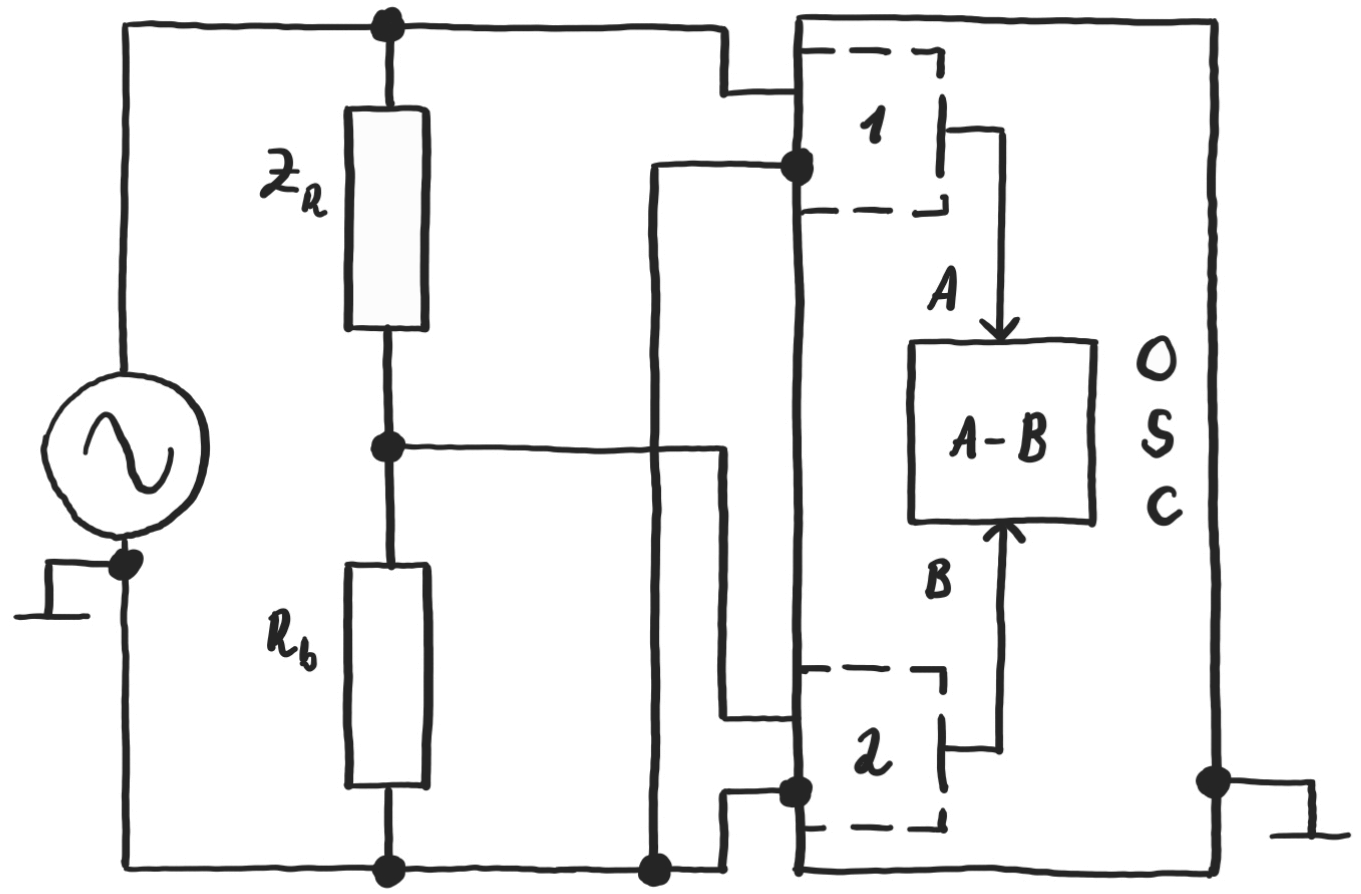
\includegraphics[width = 0.5\textwidth]{schema3b.png}
    \caption{Schéma zapojení měření impedance osciloskopem}
\end{figure}

\section{Výsledky měření}
 
\subsection{Tabulky}

\begin{table}[H]
    \centering
    \caption{Naměřené a vypočítané hodnoty měření Ohmovou metodou ($R_b = 10 \Omega$)}
    \begin{tabular}{cccccc}
        \toprule
        $f$     & $U_r$   & $U_b$   & $I$    & $Z$     & $\phi$     \\
        $[Hz]$    & $[mV]$   & $[mV]$   & $[mA]$   & $[\Omega]$     & $[\degree]$     \\
        \midrule
        10    & 23,8 & 53,3 & 5,33 & 4,47  & 5,73  \\
        20    & 24,5 & 53,3 & 5,33 & 4,60  & 13    \\
        50    & 26,9 & 52,9 & 5,29 & 5,09  & -3,2  \\
        100   & 43,3 & 51,7 & 5,17 & 8,38  & 39,4  \\
        200   & 26,1 & 53,3 & 5,33 & 4,90  & -13   \\
        500   & 27,8 & 53,2 & 5,32 & 5,23  & 14,9  \\
        1000  & 35,6 & 52,4 & 5,24 & 6,79  & 28,8  \\
        2000  & 52,5 & 50,2 & 5,02 & 10,46 & 33,4  \\
        5000  & 81   & 44,3 & 4,43 & 18,28 & 0,7   \\
        10000 & 52,3 & 49,5 & 4,95 & 10,57 & -22,3 \\
        20000 & 36,5 & 51,2 & 5,12 & 7,13  & 1,4  \\
        \bottomrule
    \end{tabular}
\end{table}

\begin{table}[H]
    \centering
    \caption{Automatizované měření impedance reproduktoru metodou tří voltmetrů (otevřený nátrubek bassreflexu)}
    \begin{tabular}{cccccc}
        \toprule
        Kmitočet   & \begin{tabular}[c]{@{}c@{}}Napětí na výstupu\\      generátoru\end{tabular} & \begin{tabular}[c]{@{}c@{}}Napětí na sériovém\\      rezistoru\end{tabular} & \begin{tabular}[c]{@{}c@{}}Napětí\\      na reproduktoru\end{tabular} & \begin{tabular}[c]{@{}c@{}}Modul\\      impedance\end{tabular} & \begin{tabular}[c]{@{}c@{}}Fáze\\      impedance\end{tabular} \\
        $f$ {[}Hz{]} & $U_c$ {[}V{]}                                                                  & $U_b$  {[}V{]}                                                                 & $U_r$  {[}V{]}                                                           & $|Z|$ {[}$\Omega${]}                                                    & $|\phi|$ {[}\degree{]}                                                   \\
        \midrule
        20,0       & 0,079                                                                       & 0,053                                                                       & 0,027                                                                 & 5,000                                                          & 17,2                                                          \\
        30,0       & 0,079                                                                       & 0,053                                                                       & 0,027                                                                 & 5,066                                                          & 21,9                                                          \\
        35,0       & 0,082                                                                       & 0,053                                                                       & 0,032                                                                 & 6,061                                                          & 30,5                                                          \\
        37,0       & 0,086                                                                       & 0,052                                                                       & 0,037                                                                 & 7,011                                                          & 29,3                                                          \\
        40,0       & 0,096                                                                       & 0,050                                                                       & 0,047                                                                 & 9,400                                                          & 16,5                                                          \\
        43,0       & 0,090                                                                       & 0,051                                                                       & 0,040                                                                 & 7,800                                                          & 13,3                                                          \\
        45,0       & 0,084                                                                       & 0,052                                                                       & 0,033                                                                 & 6,308                                                          & 16,2                                                          \\
        50,0       & 0,080                                                                       & 0,053                                                                       & 0,027                                                                 & 5,066                                                          & 0,0                                                           \\
        60,0       & 0,079                                                                       & 0,053                                                                       & 0,026                                                                 & 4,822                                                          & 0,0                                                           \\
        65,0       & 0,079                                                                       & 0,053                                                                       & 0,026                                                                 & 4,916                                                          & 13,7                                                          \\
        70,0       & 0,079                                                                       & 0,053                                                                       & 0,027                                                                 & 5,047                                                          & 21,0                                                          \\
        75,0       & 0,080                                                                       & 0,053                                                                       & 0,028                                                                 & 5,263                                                          & 20,8                                                          \\
        80,0       & 0,080                                                                       & 0,053                                                                       & 0,029                                                                 & 5,508                                                          & 29,6                                                          \\
        90,0       & 0,083                                                                       & 0,053                                                                       & 0,034                                                                 & 6,389                                                          & 34,5                                                          \\
        100,0      & 0,089                                                                       & 0,052                                                                       & 0,043                                                                 & 8,273                                                          & 41,8                                                          \\
        110,0      & 0,108                                                                       & 0,049                                                                       & 0,066                                                                 & 13,442                                                         & 40,9                                                          \\
        115,0      & 0,126                                                                       & 0,045                                                                       & 0,084                                                                 & 18,584                                                         & 26,8                                                          \\
        120,0      & 0,137                                                                       & 0,042                                                                       & 0,095                                                                 & 22,619                                                         & 0,0                                                           \\
        125,0      & 0,125                                                                       & 0,045                                                                       & 0,084                                                                 & 18,792                                                         & 29,0                                                          \\
        130,0      & 0,109                                                                       & 0,048                                                                       & 0,066                                                                 & 13,693                                                         & 35,2                                                          \\
        140,0      & 0,091                                                                       & 0,051                                                                       & 0,045                                                                 & 8,755                                                          & 38,6                                                          \\
        160,0      & 0,082                                                                       & 0,053                                                                       & 0,031                                                                 & 5,898                                                          & 26,6                                                          \\
        180,0      & 0,080                                                                       & 0,053                                                                       & 0,028                                                                 & 5,188                                                          & 17,0                                                          \\
        200,0      & 0,079                                                                       & 0,053                                                                       & 0,026                                                                 & 4,897                                                          & 12,3                                                          \\
        300,0      & 0,079                                                                       & 0,054                                                                       & 0,025                                                                 & 4,748                                                          & 0,0                                                           \\
        400,0      & 0,080                                                                       & 0,053                                                                       & 0,027                                                                 & 4,981                                                          & 0,0                                                           \\
        500,0      & 0,080                                                                       & 0,053                                                                       & 0,028                                                                 & 5,206                                                          & 20,8                                                          \\
        750,0      & 0,083                                                                       & 0,053                                                                       & 0,032                                                                 & 5,951                                                          & 23,8                                                          \\
        1000,0     & 0,085                                                                       & 0,053                                                                       & 0,036                                                                 & 6,755                                                          & 32,0                                                          \\
        1500,0     & 0,091                                                                       & 0,052                                                                       & 0,044                                                                 & 8,494                                                          & 36,6                                                          \\
        2000,0     & 0,098                                                                       & 0,051                                                                       & 0,053                                                                 & 10,375                                                         & 36,2                                                          \\
        2500,0     & 0,105                                                                       & 0,049                                                                       & 0,061                                                                 & 12,358                                                         & 34,9                                                          \\
        3000,0     & 0,112                                                                       & 0,048                                                                       & 0,067                                                                 & 13,987                                                         & 26,2                                                          \\
        3500,0     & 0,118                                                                       & 0,047                                                                       & 0,074                                                                 & 15,914                                                         & 24,0                                                          \\
        4000,0     & 0,122                                                                       & 0,045                                                                       & 0,078                                                                 & 17,181                                                         & 17,9                                                          \\
        4500,0     & 0,125                                                                       & 0,045                                                                       & 0,081                                                                 & 18,161                                                         & 11,7                                                          \\
        5000,0     & 0,125                                                                       & 0,044                                                                       & 0,081                                                                 & 18,243                                                         & 9,6                                                           \\
        6000,0     & 0,121                                                                       & 0,045                                                                       & 0,077                                                                 & 17,073                                                         & 16,0                                                          \\
        7000,0     & 0,115                                                                       & 0,046                                                                       & 0,070                                                                 & 15,086                                                         & 18,2                                                          \\
        8000,0     & 0,109                                                                       & 0,048                                                                       & 0,063                                                                 & 13,298                                                         & 21,5                                                          \\
        9000,0     & 0,104                                                                       & 0,049                                                                       & 0,057                                                                 & 11,790                                                         & 21,8                                                          \\
        10000,0    & 0,100                                                                       & 0,049                                                                       & 0,052                                                                 & 10,607                                                         & 21,6                                                          \\
        12500,0    & 0,093                                                                       & 0,051                                                                       & 0,044                                                                 & 8,733                                                          & 21,2                                                          \\
        15000,0    & 0,090                                                                       & 0,051                                                                       & 0,040                                                                 & 7,765                                                          & 13,3                                                          \\
        17500,0    & 0,089                                                                       & 0,051                                                                       & 0,037                                                                 & 7,290                                                          & 0,0                                                           \\
        20000,0    & 0,088                                                                       & 0,051                                                                       & 0,037                                                                 & 7,135                                                          & 0,0                                                          \\
        \bottomrule
    \end{tabular}
\end{table}

\begin{table}[H]
    \centering
    \caption{Automatizované měření impedance reproduktoru metodou tří voltmetrů (uzavřený nátrubek bassreflexu)}
    \begin{tabular}{cccccc}
        \toprule
        Kmitočet   & \begin{tabular}[c]{@{}c@{}}Napětí na výstupu\\      generátoru\end{tabular} & \begin{tabular}[c]{@{}c@{}}Napětí na sériovém\\      rezistoru\end{tabular} & \begin{tabular}[c]{@{}c@{}}Napětí\\      na reproduktoru\end{tabular} & \begin{tabular}[c]{@{}c@{}}Modul\\      impedance\end{tabular} & \begin{tabular}[c]{@{}c@{}}Fáze\\      impedance\end{tabular} \\
        $f$ {[}Hz{]} & $U_c$ {[}V{]}                                                                  & $U_b$  {[}V{]}                                                                 & $U_r$  {[}V{]}                                                           & $|Z|$ {[}$\Omega${]}                                                    & $|\phi|$ {[}\degree{]}                                                   \\
        \midrule
        20,0    & 0,079 & 0,053 & 0,027 & 4,991  & 14,9 \\
30,0    & 0,079 & 0,053 & 0,026 & 4,962  & 10,6 \\
35,0    & 0,079 & 0,053 & 0,026 & 4,812  & 0,0  \\
37,0    & 0,078 & 0,053 & 0,026 & 4,803  & 18,5 \\
40,0    & 0,078 & 0,053 & 0,026 & 4,784  & 17,5 \\
43,0    & 0,078 & 0,053 & 0,026 & 4,822  & 19,5 \\
45,0    & 0,078 & 0,053 & 0,026 & 4,822  & 19,5 \\
50,0    & 0,079 & 0,053 & 0,026 & 4,878  & 10,6 \\
60,0    & 0,079 & 0,053 & 0,027 & 5,103  & 23,4 \\
65,0    & 0,080 & 0,053 & 0,028 & 5,244  & 19,9 \\
70,0    & 0,080 & 0,053 & 0,029 & 5,470  & 28,4 \\
75,0    & 0,081 & 0,053 & 0,031 & 5,763  & 30,3 \\
80,0    & 0,082 & 0,053 & 0,033 & 6,132  & 33,9 \\
90,0    & 0,086 & 0,053 & 0,039 & 7,390  & 39,7 \\
100,0   & 0,096 & 0,051 & 0,053 & 10,294 & 43,9 \\
110,0   & 0,124 & 0,046 & 0,083 & 18,202 & 32,2 \\
115,0   & 0,137 & 0,042 & 0,096 & 22,912 & 14,2 \\
120,0   & 0,130 & 0,043 & 0,090 & 20,737 & 27,7 \\
125,0   & 0,114 & 0,047 & 0,072 & 15,254 & 34,8 \\
130,0   & 0,101 & 0,050 & 0,058 & 11,593 & 39,0 \\
140,0   & 0,088 & 0,052 & 0,042 & 8,104  & 40,1 \\
160,0   & 0,081 & 0,053 & 0,031 & 5,833  & 29,7 \\
180,0   & 0,080 & 0,053 & 0,027 & 5,160  & 13,5 \\
200,0   & 0,079 & 0,053 & 0,026 & 4,906  & 10,6 \\
300,0   & 0,079 & 0,053 & 0,025 & 4,757  & 0,0  \\
400,0   & 0,080 & 0,053 & 0,027 & 4,963  & 0,0  \\
500,0   & 0,080 & 0,053 & 0,028 & 5,216  & 19,9 \\
750,0   & 0,083 & 0,053 & 0,032 & 5,962  & 23,1 \\
1000,0  & 0,085 & 0,053 & 0,036 & 6,755  & 32,0 \\
1500,0  & 0,091 & 0,052 & 0,044 & 8,511  & 36,2 \\
2000,0  & 0,098 & 0,051 & 0,053 & 10,396 & 35,9 \\
2500,0  & 0,105 & 0,049 & 0,061 & 12,383 & 34,5 \\
3000,0  & 0,112 & 0,048 & 0,067 & 13,987 & 26,2 \\
3500,0  & 0,118 & 0,046 & 0,074 & 15,948 & 23,6 \\
4000,0  & 0,122 & 0,045 & 0,078 & 17,219 & 17,3 \\
4500,0  & 0,125 & 0,045 & 0,081 & 18,161 & 11,7 \\
5000,0  & 0,125 & 0,044 & 0,081 & 18,284 & 8,3  \\
6000,0  & 0,121 & 0,045 & 0,077 & 17,111 & 15,2 \\
7000,0  & 0,115 & 0,046 & 0,070 & 15,119 & 17,5 \\
8000,0  & 0,109 & 0,048 & 0,063 & 13,277 & 20,9 \\
9000,0  & 0,104 & 0,049 & 0,057 & 11,770 & 21,2 \\
10000,0 & 0,100 & 0,049 & 0,052 & 10,629 & 21,0 \\
12500,0 & 0,093 & 0,050 & 0,044 & 8,730  & 19,8 \\
15000,0 & 0,090 & 0,051 & 0,040 & 7,765  & 13,3 \\
17500,0 & 0,089 & 0,051 & 0,037 & 7,290  & 0,0  \\
20000,0 & 0,088 & 0,051 & 0,037 & 7,135  & 0,0 \\
        \bottomrule
    \end{tabular}
\end{table}

\subsection{Grafy}

\begin{figure}[H]
    \centering
    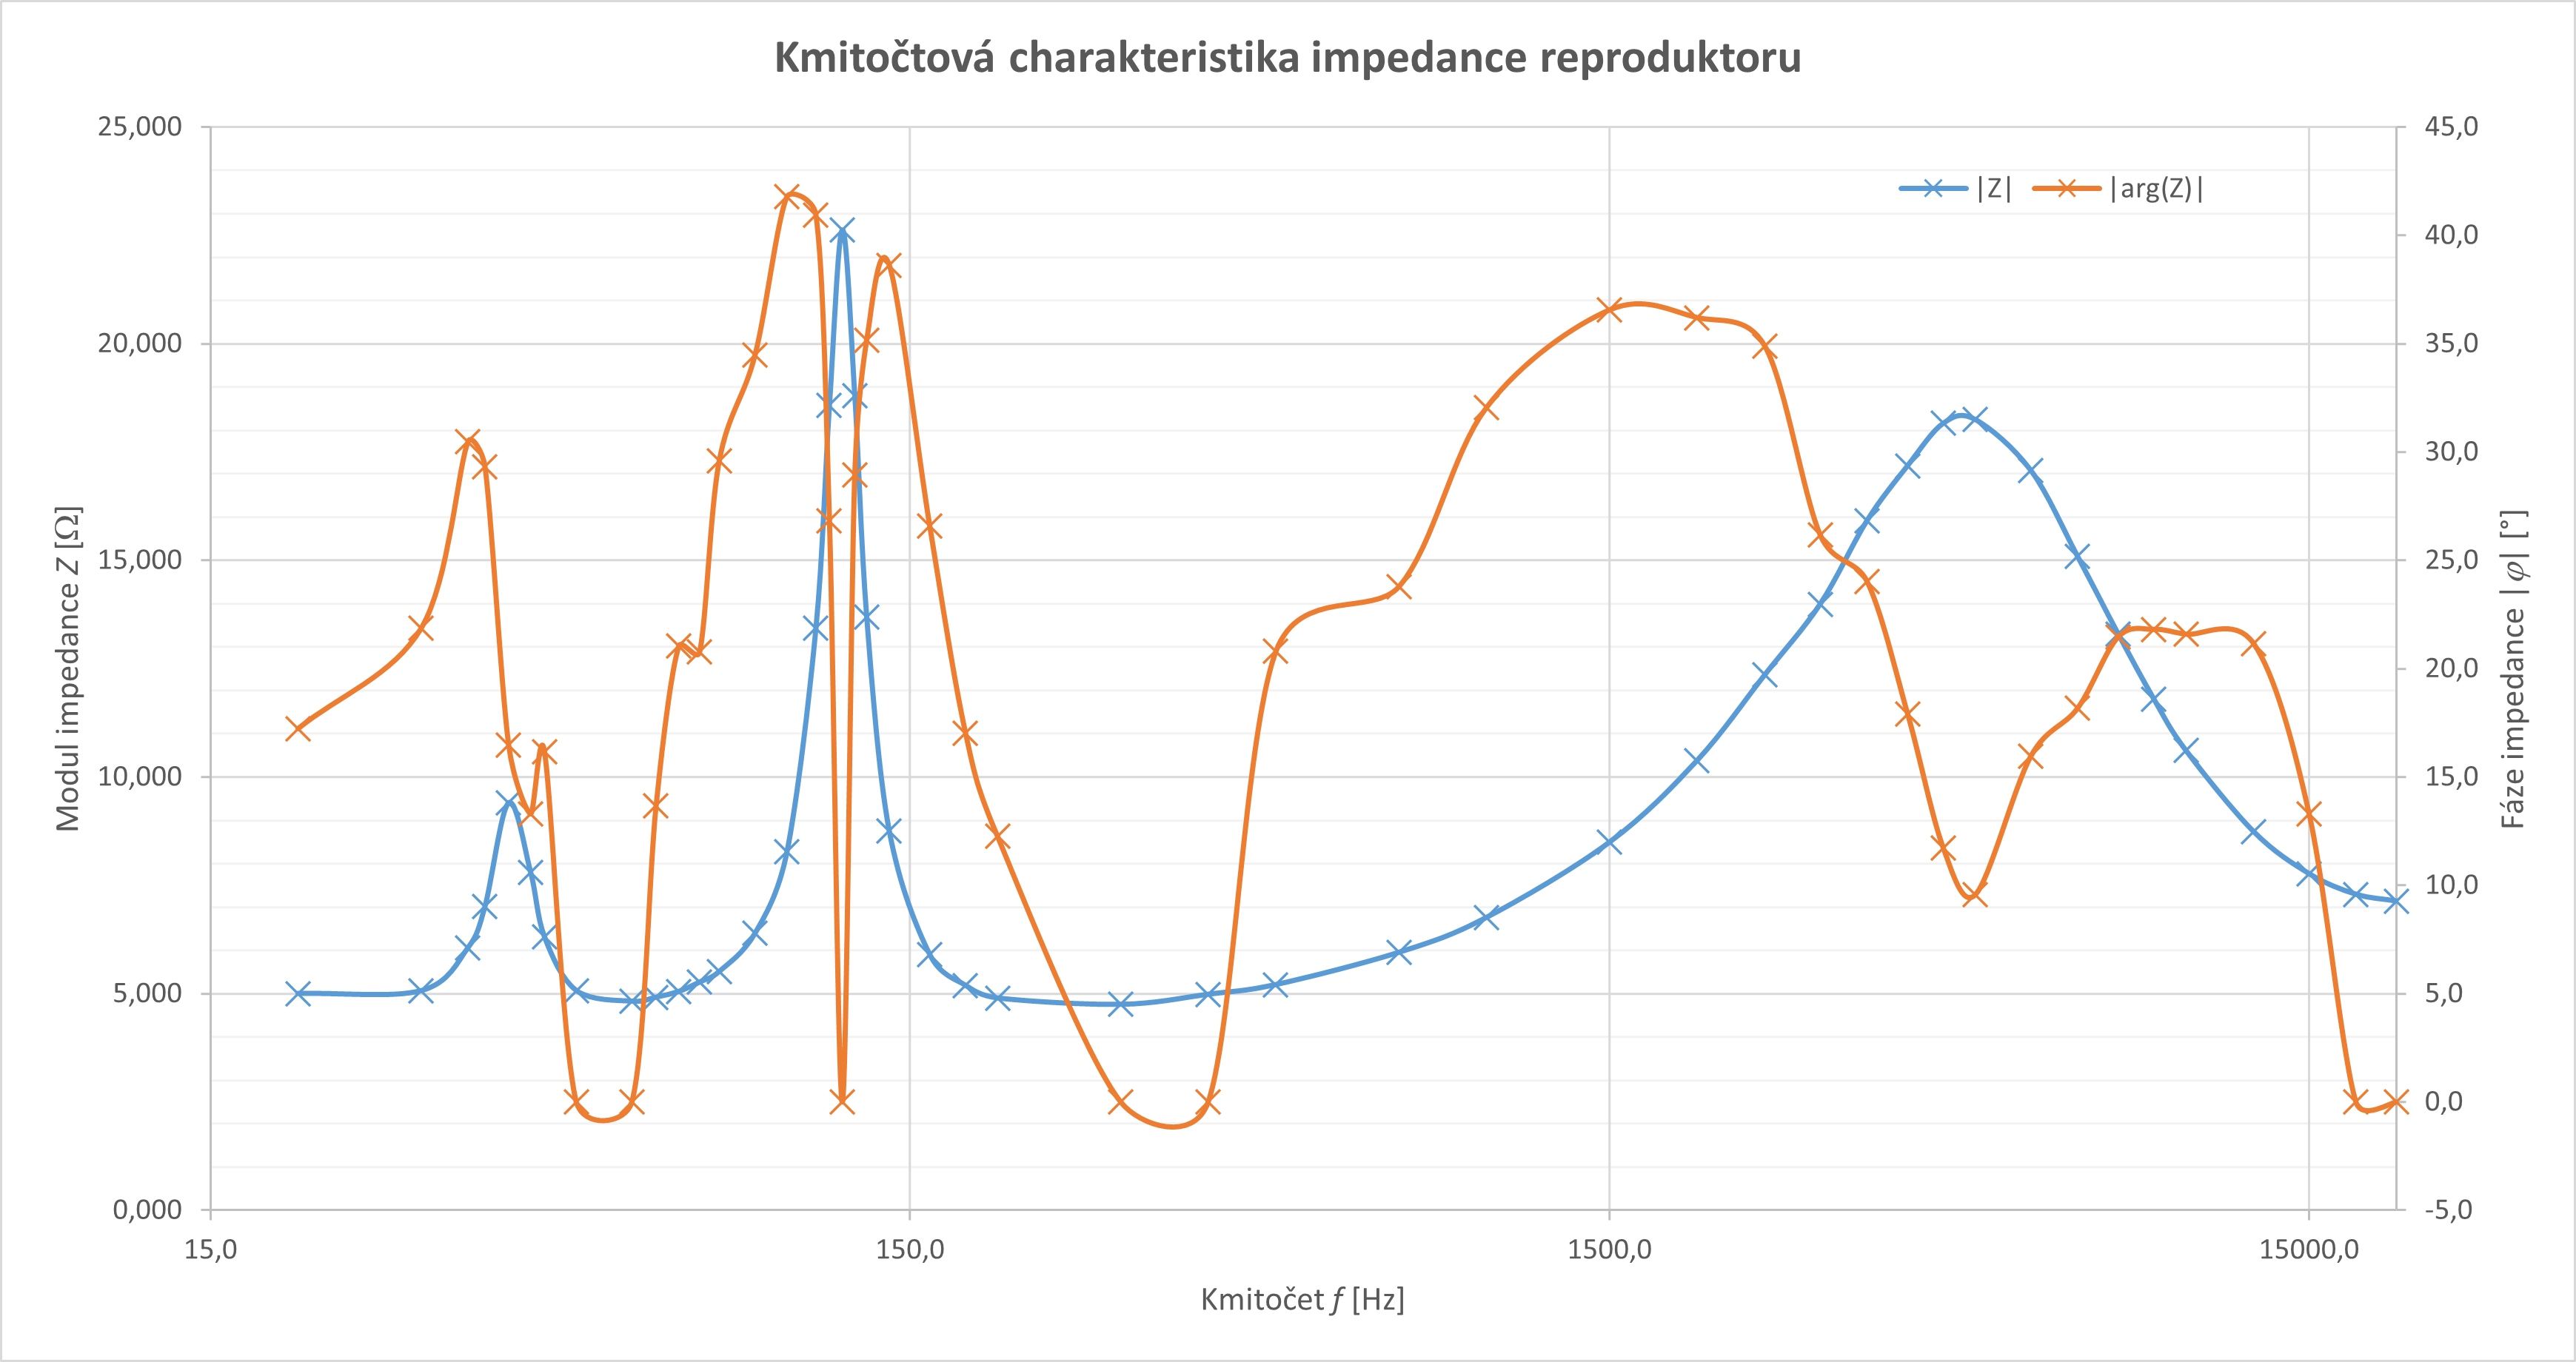
\includegraphics[width=\textwidth]{graf3b_otevreny.png}
    \caption{Kmitočtová charakteristika impedance reproduktoru (otevřený nátrubek bassreflexu)}
\end{figure}

\begin{figure}[H]
    \centering
    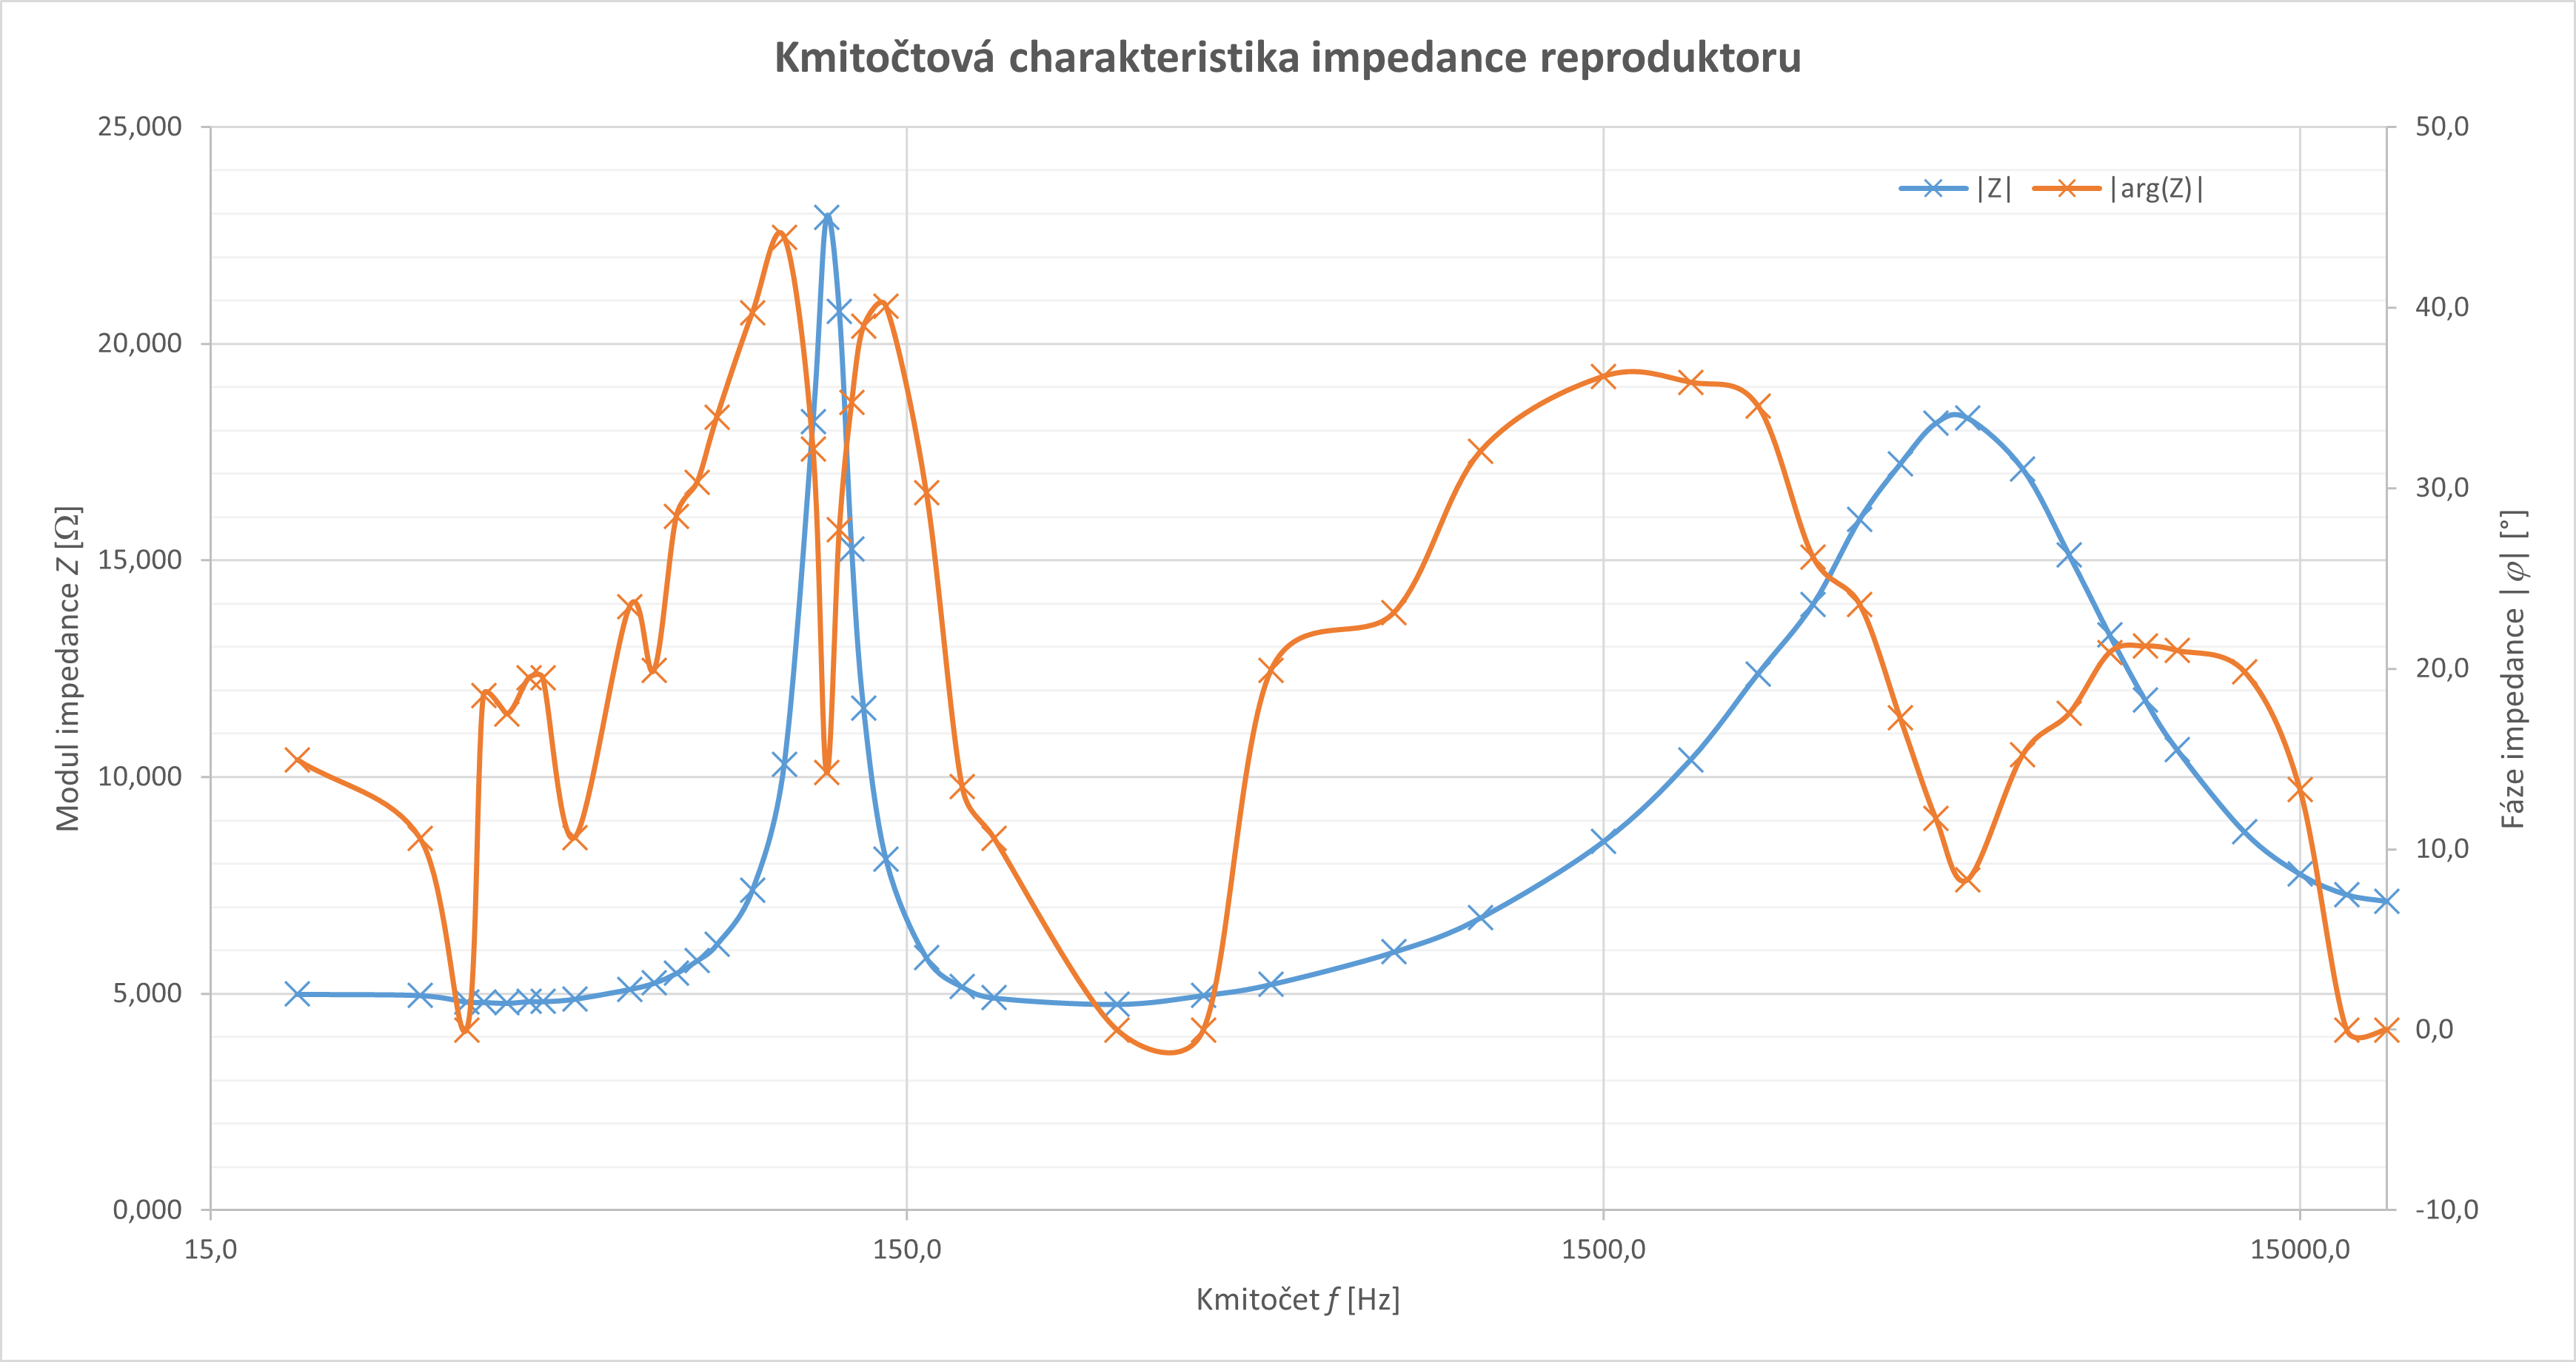
\includegraphics[width=\textwidth]{graf3b_zavreny.png}
    \caption{Kmitočtová charakteristika impedance reproduktoru (uzavřený nátrubek bassreflexu)}
\end{figure}

\break

\subsection{Příklady výpočtu}

\begin{enumerate}
    \item Elektrický proud tekoucí reproduktorem:
    \begin{multline*}
        I = \frac{U_b}{R_b} = \frac{53,3 \cdot 10^{-3} V}{10 \Omega} = 5,33 \cdot 10^{-3} A = \underline{\underline{5,33\ mA}} \hfill
    \end{multline*}

    \item Modul impedance reproduktoru:
    \begin{multline*}
        Z = \frac{U_r}{I} = \frac{23,8 \cdot 10^{-3} V}{5,33 \cdot 10^{-3} A} = \underline{\underline{4,47 \Omega}} \hfill
    \end{multline*}
\end{enumerate}

\section{Seznam použitých přístrojů}

\begin{itemize}
    \item Počítač vybaven programem HP VEE 9.0
    \item Reproduktor konektorem RCA/Cinch, s pěnovou ucpávkou nátrubku bassreflexu
    \item Osciloskop Agilent DSO-X 3014A
    \item Laboratorní přípravek se sériovým odporem 10 $\Omega$
\end{itemize}

\section{Závěr}

Z kmitočtových charakteristiky impedance reproduktoru s otevřeným nátrubkem bassreflexu jsme určili stejnosměrný odpor (určený na počátku kmitočtové charakteristiky impedance) na hodnotu 5 $\Omega$.
Jmenovitou impedanci reproduktoru (definována jako nejnižší hodnota impedance v pracovním kmitočtovém pásmu) jsme určili na hodnotu 4,748 $\Omega$.
Rezonanční kmitočty (lokální maxima na kmitočtové závislosti impedance) reproduktoru leží na hodnotách kmitočtu 40 Hz, 120 Hz a 5000 Hz.

U reproduktoru s uzavřeným nátrubkem bassreflexu jsme určili stejnosměrný odpor 4,991 $\Omega$.
Jmenovitou impedanci reproduktoru jsme určili na hodnotu 4,757 $\Omega$.
Rezonanční kmitočty reproduktoru leží na hodnotách kmitočtu  115 Hz a 5000 Hz.

Z úbytku počtu rezonančních kmitočtů při uzavření nátrubku bassreflexu vyplývá, že uzavřením zamezujeme reproduktoru rezonovat na nejnižších frekvencích.

Hodnoty ručního měření Ohmovou metodou se od hodnot automatizovaného měření metodou tří voltmetru příliš neliší.
Případné nepřesnosti lze vysvětlit systematickou chybou při odčítání hodnot, případně rozdílem v použitých metodách měření.
Výhoda Ohmovy metody je, že je díky ní možné poznat znaménko měřeného fázového posunu impedance.

\end{document}